\documentclass[10pt]{article}
\usepackage[a4paper, margin=2cm]{geometry}
%\usepackage{fullpage}
\usepackage[T1]{fontenc}
\usepackage[utf8]{inputenc}
\usepackage{graphicx}
\usepackage{mathpazo}
\pagenumbering{arabic}
\usepackage{siunitx}
\usepackage{amsmath}
\usepackage{mathtools} % Para poder usar "\Aboxed"
\usepackage{cancel} % Para usar "\cancel", de https://tex.stackexchange.com/questions/537955/how-do-cross-out-text-in-math-mode
\usepackage{multicol}
\usepackage[spanish]{babel}
\usepackage{steinmetz}
\DeclareSIUnit\voltampere{VA}
\DeclareSIUnit\var{VAr}
\setlength\parindent{0pt} % no indent

% Numbering pages on the right footer:
% (https://tex.stackexchange.com/questions/153167/how-to-set-page-number-at-right-footer)
\usepackage{fancyhdr}
% Turn on the style
\pagestyle{fancy}
\fancyhf{} % sets both header and footer to nothing
\renewcommand{\headrulewidth}{0pt} % To remove the top horizontal line created by default by "fancyhdr", from here: https://tex.stackexchange.com/questions/13896/how-to-remove-the-top-horizontal-bar-in-fancyhdr
% Set the right side of the footer to be the page number
\fancyfoot[R]{\thepage}


\usepackage{minibox} % Para poder partir el texto en 2 líneas usando "underbrace" u "overbrace", info aquí: https://tex.stackexchange.com/questions/8680/how-can-i-insert-a-newline-in-a-framebox


\usepackage{xparse} % For "overbrace/underbrace but with an arrow instead", from https://tex.stackexchange.com/questions/8720/overbrace-underbrace-but-with-an-arrow-instead

% Para poner flechas sobre los signos de igual, de aquí: https://tex.stackexchange.com/questions/8720/overbrace-underbrace-but-with-an-arrow-instead
\NewDocumentCommand{\overarrow}{O{=} O{\uparrow} m}{%
  \overset{\makebox[0pt]{\begin{tabular}{@{}c@{}}#3\\[0pt]\ensuremath{#2}\end{tabular}}}{#1}
}
\NewDocumentCommand{\underarrow}{O{=} O{\downarrow} m}{%
  \underset{\makebox[0pt]{\begin{tabular}{@{}c@{}}\ensuremath{#2}\\[0pt]#3\end{tabular}}}{#1}
}



\begin{document}

\large{\textbf{Ejercicio 9 de la colección de problemas}}

\vspace{3mm}
\large{\textbf{Enunciado}}:

\vspace{5mm}

En el circuito de la figura, los condensadores se conectaron sin carga. Mediante el método de las mallas, se pide determinar:
\begin{enumerate}
    \item Intensidades de corriente señaladas
    \item Potenciales en los puntos A, B, C y D
    \item Polaridades, cargas, y energía almacenada en los condensadores
    \item Balance de potencias
\end{enumerate}

\vspace{-3mm}
\begin{minipage}[c]{0.2\linewidth}
  \begin{align*}
    \epsilon_{1}&=\qty{118}{\volt}\\
    \epsilon_{2}&=\qty{236}{\volt}\\
    \epsilon_{3}&=\qty{118}{\volt}\\
    R_{1}&= \qty{4}{\ohm}\\
    R_{2}&=R_{3}=\qty{1}{\ohm}\\
    R_{4}&= \qty{3}{\ohm}\\
    R_{5}&= \qty{2}{\ohm}\\
    C_{1}&=C_{2}=C_{3}=\qty{2}{\micro\farad}\\
    L_1 &= L_2 = L_3 = \qty{1}{\milli\henry}\\
  \end{align*}
\end{minipage}
\begin{minipage}[c]{0.8\linewidth}
  \hspace{-12mm}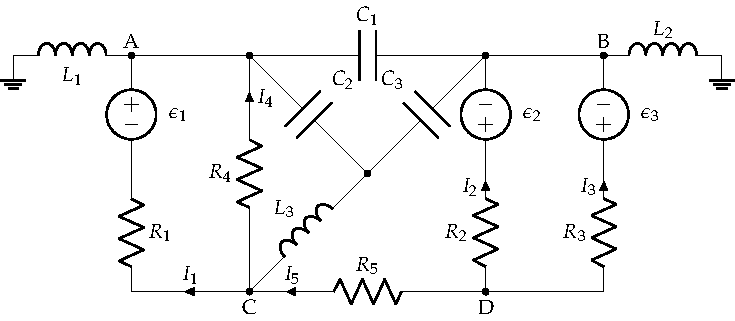
\includegraphics[scale=1.15]{figs/mallas_condensadores.pdf}
\end{minipage}

\vspace{3mm}

\hrulefill

\vspace{5mm}
\textbf{Solución}:
\vspace{4mm}

Se sustituyen los condensadores y las bobinas por sus equivalentes en un circuito de corriente continua (circuito abierto y cortocircuito, respectivamente). Por otro lado, dado que hay dos tomas de tierra en el esquema, esto no implica que haya dos referencias de potencial distintas: simplemente indica que esos dos puntos están cortocircuitados. En el circuito resultante, se definen tres corrientes de malla, como se muestra en el circuito de la figura:

%\vspace{1mm}
\begin{center}
  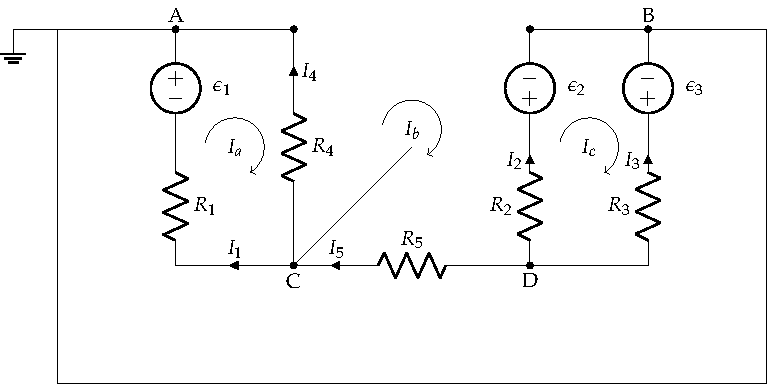
\includegraphics[scale=1.08]{figs/mallas_condensadores_sol.pdf}
\end{center}

\vspace{1mm}
(la malla $b$ puede definirse de esta forma porque los puntos A y B están cortocircuitados)

\vspace{5mm}
Usamos la ecuación general del método de mallas:    
\begin{equation*}
    \begin{bmatrix}
        R_1 + R_4 & -R_4 & 0\\
        -R_4 & R_4 + R_5 + R_2 & -R_{2}\\
        0 & -R_2 & R_2 + R_3
    \end{bmatrix} \cdot %
    \begin{bmatrix}
        I_{a}\\
        I_{b}\\
        I_{c}
    \end{bmatrix} = %
    \begin{bmatrix}
        \epsilon_1\\
        \epsilon_2\\
        \epsilon_3 - \epsilon_2
    \end{bmatrix}
\end{equation*} 

\begin{equation*}
    \begin{bmatrix}
        7 & -3 & 0\\
        -3 & 6 & -1\\
        0 & -1 & 2
    \end{bmatrix} \cdot %
    \begin{bmatrix}
        I_{a}\\
        I_{b}\\
        I_{c}
    \end{bmatrix} = %
    \begin{bmatrix}
        118\\
        236\\
        -118
    \end{bmatrix}
\end{equation*}  

Cuya solución es:

\vspace{-3mm}
\begin{equation*}
    I_a = \qty{40}{\ampere} \; , \qquad\qquad
    I_b = \qty{54}{\ampere} \; , \qquad\qquad
    I_c = -\qty{32}{\ampere}
\end{equation*}

\vspace{2mm}
Por tanto, las corrientes indicadas en el circuito son:

\vspace{-1mm}
\begin{equation*}
    \boxed{I_1 = \qty{40}{\ampere}}  \; , \qquad
    \boxed{I_2 = \qty{-86}{\ampere}}  \; , \qquad
    \boxed{I_3 = \qty{32}{\ampere}}  \; , \qquad
    \boxed{I_4 = \qty{14}{\ampere}}  \; , \qquad
    \boxed{I_5 = \qty{54}{\ampere}}
\end{equation*}

\vspace{4mm}
Los potenciales en los puntos indicados son:

\vspace{-2mm}
\begin{equation*}
    \boxed{U_A = \qty{0}{\volt}}  \; , \qquad
    \boxed{U_B = \qty{0}{\volt}}  \; , \qquad
    U_C = I_4 \cdot R_4 = \boxed{\qty{42}{\volt}}  \; , \qquad
    U_D = I_5 \cdot R_5 + U_c = \boxed{\qty{150}{\volt}}\\
\end{equation*}

\vspace{3mm}
Por tanto, las polaridades de los condensadores y sus valores de tensión son los siguientes:

\vspace{-3mm}
\begin{eqnarray*}
    U_{C_1} = U_{BA} & = & \qty{0}{\volt}\\
    q_1 = C_1 \cdot U_{C_1} & = & \boxed{\qty{0}{\coulomb}}\\
    E_{C_1} = \frac{1}{2} C_1 \cdot (U_{C_1})^2 & = & \boxed{\qty{0}{\joule}}
\end{eqnarray*}

\vspace{-4mm}
\begin{eqnarray*}
    U_{C_2} = U_{CA} & = & \qty{42}{\volt}\\
    q_2 = C_2 \cdot U_{C_2} & = & \boxed{\qty{84}{\micro\coulomb}}\\
    E_{C_2} = \frac{1}{2} C_2 \cdot (U_{C_2})^2 & = & \boxed{\qty{1.76}{\milli\joule}}
\end{eqnarray*}

\vspace{-4mm}
\begin{eqnarray*}
    U_{C_3} = U_{CB} & = & \qty{42}{\volt}\\
    q_3 = C_3 \cdot U_{C_3} & = & \boxed{\qty{84}{\micro\coulomb}}\\
    E_{C_3} = \frac{1}{2} C_3 \cdot (U_{C_3})^2 & = & \boxed{\qty{1.76}{\milli\joule}}
\end{eqnarray*}

\vspace{5mm}
Finalmente, podemos formular el balance de potencias como potencia entregada por los elementos activos frente a potencia consumida por los elementos pasivos:

\vspace{1mm}
\begin{itemize}
    \item La potencia total entregada por los elementos activos es $\qty{21240}{\watt}$:
\end{itemize}

\vspace{-7mm}
\begin{eqnarray*}
P_{\epsilon_1} = \epsilon_1 \cdot I_1 & = & \qty{4720}{\watt}\\
P_{\epsilon_2} = \epsilon_2 \cdot (-I_2) & = & \qty{20296}{\watt}\\
P_{\epsilon_3} = \epsilon_3 \cdot (-I_3) & = & \qty{-3776}{\watt}
\end{eqnarray*}

\vspace{1mm}
\begin{itemize}
    \item La potencia total consumida por los elementos pasivos también es $\qty{21240}{\watt}$:
\end{itemize}

\vspace{-6mm}
\begin{eqnarray*}
P_{R_1} = R_1 \cdot (I_1)^2 & = & \qty{6400}{\watt}\\
P_{R_2} = R_2 \cdot (I_2)^2 & = & \qty{7396}{\watt}\\
P_{R_3} = R_3 \cdot (I_3)^2 & = & \qty{1024}{\watt}\\
P_{R_4} = R_4 \cdot (I_4)^2 & = & \qty{588}{\watt}\\
P_{R_5} = R_5 \cdot (I_5)^2 & = & \qty{5832}{\watt}
\end{eqnarray*}

\end{document}
